\chapter{Appendix: Three-Node Model Formulation}
\section{Model}
\begin{center}
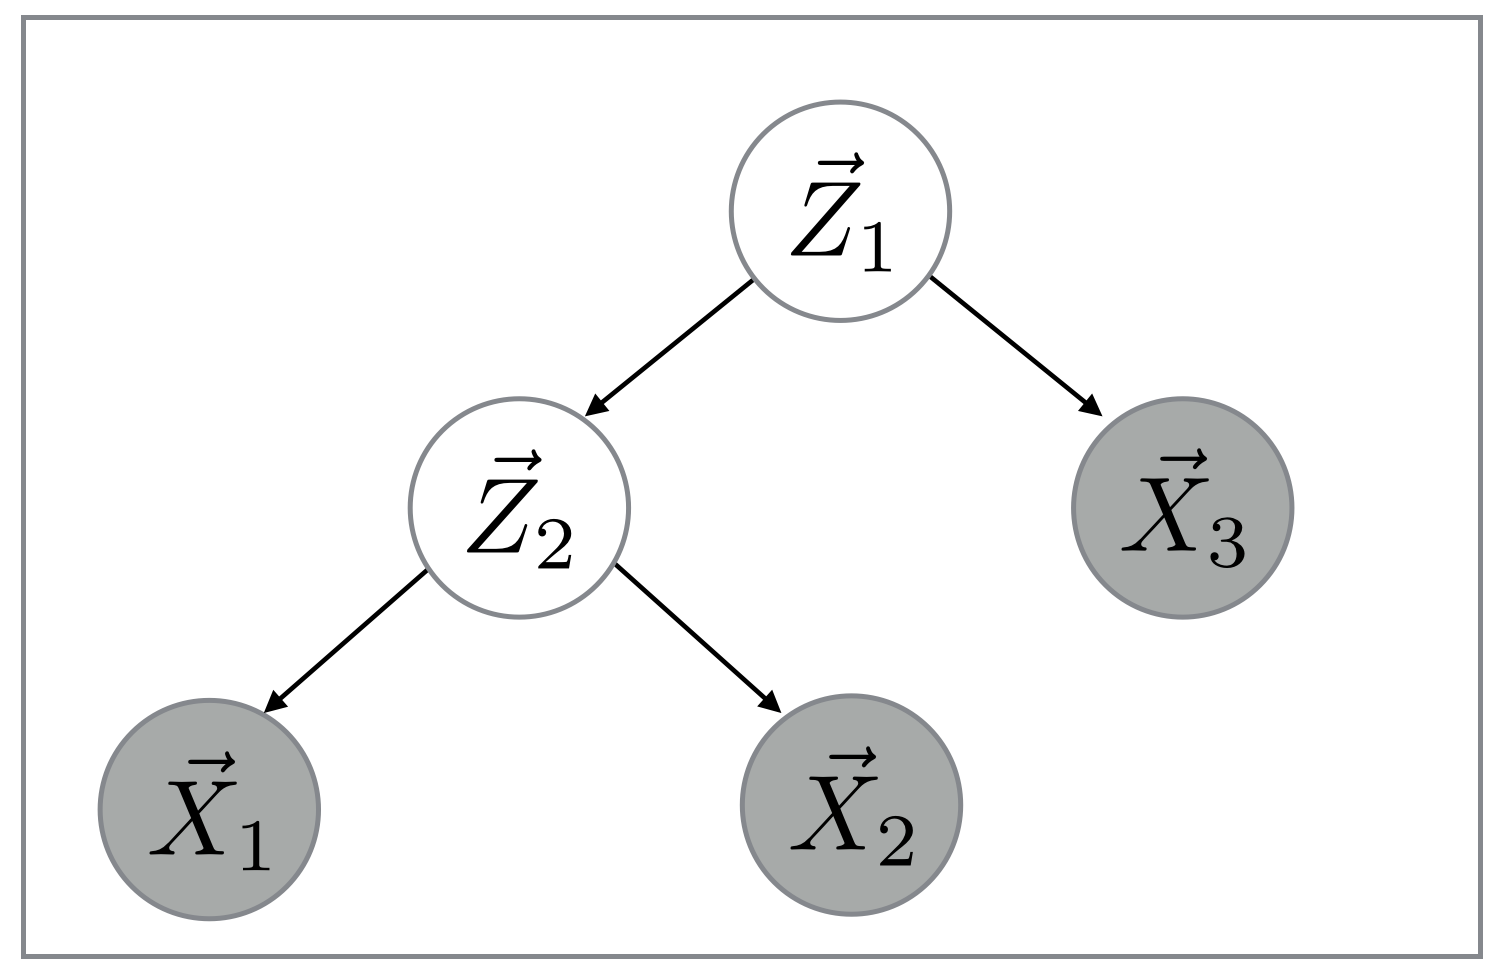
\includegraphics[width=\textwidth/3]{MFAA.png}
\end{center}
\newcommand{\fulljointp}{P \left(
  \{\x_{i,n}\}_{i=1}^3,\{ \z_{j,n}\}_{j=1}^2| \{\W_k\}_{k=0}^3,
    \{\bpsi_{\ell}\}_{\ell=0}^3 \right)}
\begin{align*}
  \fulljointp &= P(\z_1) P(\z_2 | \z_1) P(\x_1 | \z_2) P(\x_2 | \z_2)
                P(\x_3 | \z_1) \\
  \z_1 &\sim N(\vec{0}, \I ) \inreala{m}{1} \\
  \z_2| \z_1 &\sim N(\W_0 \z_1, \bpsi_0) \inreala{p_0}{1}\\
  \x_1 | \z_2 &\sim N(\W_1 \z_2, \bpsi_1) \inreala{ p_1}{1}\\
  \x_2 | \z_2 &\sim N(\W_2 \z_2, \bpsi_2) \inreala{p_2}{1} \\
  \x_3 | \z_1 &\sim N(\W_3 \z_1, \bpsi_3) \inreala{p_3}{1}
\end{align*}
%This implies the following dimensions for parameters $\W$ and $\bpsi$:
\begin{align*}
  \W_0 &\inreala{p_0}{m} &   \bpsi_0 &\inreala{p_0}{p_0} \\
  \W_1 &\inreala{p_1}{p_0} &  \bpsi_1 &\inreala{p_1}{p_1}\\
  \W_2 &\inreala{p_2}{p_0} &   \bpsi_2 &\inreala{p_2}{p_2}\\
  \W_3 &\inreala{p_3}{m} &         \bpsi_3 &\inreala{p_3}{p_3}\\  
\end{align*}


\section{Complete Log-Likelihood}
For $N$ samples, 
\begin{equation}
\begin{split}
\ell_n(\Theta) \coloneqq \sum_{n=1}^N & \log  \left( \fulljointp \right) = \\
&\sum_{n=1}^N -\frac{p_1}{2} \log (2 \pi) - \frac{1}{2} \log(|\bpsi_1|) -
\frac{1}{2} \left( \left( \x_{1,n} - \W_1 \z_{2,n} \right)^T \bpsi_1^{-1} \left(
    \x_{1,n} - \W_1 \z_{2,n} \right) \right) + \\
& -\frac{p_2}{2} \log (2 \pi) - \frac{1}{2} \log(|\bpsi_2|) -
\frac{1}{2} \left( \left( \x_{2,n} - \W_2 \z_{2,n} \right)^T \bpsi_2^{-1} \left(
    \x_{2,n} - \W_2 \z_{2,n} \right) \right) + \\
& -\frac{p_3}{2} \log (2 \pi) - \frac{1}{2} \log(|\bpsi_3|) -
\frac{1}{2} \left( \left( x_{3,n} - \W_3 \z_{1,n} \right)^T \bpsi_3^{-1} \left(
    \x_{3,n} - \W_3 \z_{1,n} \right) \right) + \\
& -\frac{p_0}{2} \log (2 \pi) - \frac{1}{2} \log(|\bpsi_0|) -
\frac{1}{2} \left( \left( \z_{2,n} - \W_0 \z_{1,n} \right)^T \bpsi_0^{-1} \left(
    \z_{2,n} - \W_0 \z_{1,n} \right) \right) + \\
& -\frac{m}{2} \log (2 \pi) - \frac{1}{2} \z_{1,n}^T \z_{1,n} 
\end{split}
\end{equation}



\newcommand{\ecll}{\ev_{\{ \z_j\}_{j=1}^2 | \{\x_i\}_{i=1}^3}
  \left[ \sum_{n=1}^N \log \left( \fulljointp \right) \right] }
\begin{equation}
\begin{split}
\Rightarrow & \ecll= \\
& \sum_{n=1}^N - \frac{p_1}{2} \log (2\pi) - \frac{1}{2} \log( |\bpsi_1| ) -
\frac{1}{2} \left(
  \x_{1,n}^T \bpsi_1^{-1} \x_{1,n} - 2 \x_{1,n}^T    \bpsi_1^{-1} \W_1 \ev[ \z_{2,n}] +
  \Tr \left( \ev[\z_{2,n} \z_{2,n}^T ] \W_1^T  \bpsi_1^{-1}
    \W_1\right) \right)\\
& - \frac{p_2}{2} \log (2\pi) - \frac{1}{2} \log( |\bpsi_2| ) -
\frac{1}{2} \left(
\x_{2,n}^T \bpsi_2^{-1} \x_{2,n} - 2 \x_{2,n}^T    \bpsi_2^{-1} \W_2 \ev[\z_{2,n}] +
  \Tr \left( \ev[\z_{2,n} \z_{2,n}^T ] \W_2^T  \bpsi_2^{-1}
    \W_2\right) \right)\\
& - \frac{p_3}{2} \log (2\pi) - \frac{1}{2} \log( |\bpsi_3| ) -
\frac{1}{2} \left(
\x_{3,n}^T \bpsi_3^{-1} \x_{3,n} - 2 \x_{3,n}^T    \bpsi_3^{-1} \W_3 \ev[\z_{1,n} ]+
  \Tr \left( \ev[\z_{1,n} \z_{1,n}^T ] \W_3^T  \bpsi_3^{-1}
    \W_3\right) \right)\\
& - \frac{p_0}{2} \log (2\pi) - \frac{1}{2} \log( |\bpsi_0| ) -
\frac{1}{2} \left(
\Tr \left( \ev [\z_{2,n} \z_{2,n}^T] \bpsi_0^{-1} \right)  - 2 \Tr \left( \ev[\z_{1,n}\z_{2,n}^T]
  \bpsi_0^{-1} \W_0 \right) +
  \Tr \left( \ev[\z_{1,n} \z_{1,n}^T ] \W_0^T  \bpsi_0^{-1}
    \W_0\right) \right)\\
& -\frac{m}{2} \log( 2 \pi) - \frac{1}{2} \ev [ \z_{1,n}^T \z_{1,n}]
\end{split}
\end{equation}
\pagebreak
\section{M-Step: Finding Critical Points}
\subsection{$\W$}

% W_0
\begin{align*}
  &\frac{  \partial }{\partial \W_0} \ecll \\
  &=  \sum_{n=1}^N \frac{\partial}{\partial \W_0} \Tr \left(\ev [\z_{1,n} \z_{2,n}^T]
      \bpsi_0^{-1} \W_0 \right) - \frac{1}{2} \frac{\partial}{\partial
      \W_0 }\Tr \left( \ev [ \z_{1,n}
    \z_{1,n}^T] \W_0^T \bpsi_0^{-1} \W_0 \right) \\
  &=  \ev [\z_{1,n} \z_{2,n}^T] \bpsi_0^{-1} - \ev [\z_{1,n} \z_{1,n}^T] \W_0^T
    \bpsi_0^{-1}\\
   \Rightarrow \Aboxed{ \hat{\W_0^T}_{\text{MLE}} &= \left(
                                                    \sum_{n=1}^N \ev [\z_{1,n} \z_{1,n}^T]
      \right)^{-1} \left( \sum_{n=1}^N \ev [\z_{1,n} \z_{2,n}^T] \right)}\\
\end{align*}

\begin{align*}
  &\frac{\partial} {\partial \W_1} \ecll \\
  &= \sum_{n=1}^N \frac{\partial}{\partial \W_1} \x_{1,n}^T \bpsi_1^{-1} \W_1 \ev
    [\z_{2,n}] - \frac{1}{2} \frac{\partial}{\partial \W_1} \Tr \left( \ev
    [\z_{2,n} \z_{2,n}^T] \W_1^T \bpsi_1^{-1} \W_1 \right)\\
  &= \ev[\z_{2,n}] \x_{1,n}^T \bpsi_1^{-1} - \ev [ \z_{2,n} \z_{2,n}^T] \W_1^T
    \bpsi_1^{-1} \\
    \Rightarrow \Aboxed{ \hat{ \W_1^T }_{\text{MLE}} &= \left(
                                                       \sum_{n=1}^N
                                                       \ev [ \z_{2,n}
                                                       \z_{2,n}^T]
                                                       \right)^{-1}
                                                       \left(
                                                       \sum_{n=1}^N \ev [ \z_{2,n}]
      \x_{1,n}^T  \right)}
\end{align*}

By pattern-matching,
\begin{align*}
\Aboxed{  \hat{\W_2^T}_{\text{MLE}} &= \left( \sum_{n=1}^N \ev [ \z_{2,n} \z_{2,n}^T] \right)^{-1}
                              \left( \sum_{n=1}^N \ev [ \z_{2,n}]
                                      \x_{2,n}^T  \right)}\\
\Aboxed{    \hat{\W_3^T}_{\text{MLE}} &= \left( \sum_{n=1}^N \ev [ \z_{1,n} \z_{1,n}^T] \right)^{-1}
                              \left( \sum_{n=1}^N \ev [ \z_{1,n}] \x_{3,n}^T \right)}\\  
\end{align*}

\subsection{$\bpsi$}


\begin{align*}
  &\frac{\partial}{\partial \bpsi_0} \ecll = \\
  & \sum_{n=1}^N \left( - \frac{\partial}{\partial \bpsi_0}  \frac{1}{2} \log \left( \left|
    \bpsi_0 \right| \right) - \frac{1}{2} \frac{\partial}{\partial
    \bpsi_0}\Tr \left( \ev [\z_{2,n} \z_{2,n}^T] \bpsi_0^{-1} \right)  +
    \frac{\partial}{\partial \bpsi_0} \Tr \left( \ev [\z_{1,n} \z_{2,n}^T ]
    \bpsi_0^{-1} \W_0 \right) - \frac{1}{2} \frac{\partial}{\partial \bpsi_0} \Tr
    \left( \ev [\z_{1,n} \z_{1,n}^T] \W_0^T \bpsi_0^{-1} \W_0 \right) \right) \\
    &=\sum_{n=1}^N \left( -\frac{1}{2} \bpsi_0^{-1}  + \frac{1}{2} \bpsi_0^{-1} \ev[\z_{2,n} \z_{2,n}^T] \bpsi_0^{-1} - \bpsi_0^{-1} \ev[\z_{2,n} \z_{1,n}^T] \W_0^T
      \bpsi_0^{-1} + \frac{1}{2} \bpsi_0^{-1} \W_0 \ev [\z_{1,n} \z_{1,n}^T ] \W_0^T
      \bpsi_0^{-1}\right) \\
  \Rightarrow \hat{\bpsi_0}_{\text{MLE}} &= \frac{1}{N}  \sum_{n=1}^N \left( \ev[ \z_{2,n} \z_{2,n}^T] - 2 \ev [\z_{2,n} \z_{1,n}^T] \W_0^T +  \W_0 \ev[\z_{1,n}
    \z_{1,n}^T] \W_0^T       \right)
\end{align*}
By pattern-matching, 
\begin{align*}
 \hat{\bpsi_1}_{\text{MLE}} &=  \frac{1}{N}  \sum_{n=1}^N \left( \x_{1,n} \x_{1,n}^T - 2 \x_{1,n}
                                        \ev[\z_{2,n}^T] \W_1^T +  \W_1 \ev[\z_{2,n}
                                \z_{2,n}^T] \W_1^T      \right) \\
 \hat{\bpsi_2}_{\text{MLE}} &= \frac{1}{N}  \sum_{n=1}^N \left( \x_{2,n} \x_{2,n}^T - 2 \x_{2,n}
                                           \ev[\z_{2,n}^T] \W_2^T +  \W_2 \ev[\z_{2,n}
                                  \z_{2,n}^T] \W_2^T       \right) \\
 \hat{\bpsi_3}_{\text{MLE}} &=  \frac{1}{N}  \sum_{n=1}^N \left( \x_{3,n} \x_{3,n}^T - 2 \x_{3,n} \ev[\z_{1,n}^T] \W_3^T + \W_3 \ev[\z_{1,n}
    \z_{1,n}^T] \W_3^T      \right) \\
\end{align*}

Using a generalized EM algorithm, and therefore substituting $\W$ with
$\hat{\W}_{\text{MLE}}$ in $\hat{\bpsi}_{\text{MLE}}$:

\begin{align*}
\Aboxed{ \hat{\bpsi_0}_{\text{MLE}} &=  \frac{1}{N}  \sum_{n=1}^N \left( \ev[\z_{2,n} \z_{2,n}^T] -  \ev [\z_{2,n} \z_{1,n}^T]
                             \left( \ev [z_{1,n} \z_{1,n}^T ] \right)^{-1} \ev[
                                      \z_{1,n} \z_{2,n}^T] \right) }\\
\Aboxed{   \hat{\bpsi_1}_{\text{MLE}} &=\frac{1}{N}  \sum_{n=1}^N  \left( \x_{1,n} \x_{1,n}^T - \x_{1,n} \ev[\z_{2,n}^T]
                                        \left( \ev [\z_{2,n} \z_{2,n}^T
                                        ]\right)^{-1} \ev[\z_{2,n}]
                               \x_{1,n}^T \right)}\\
  \Aboxed{   \hat{\bpsi_2}_{\text{MLE}} &= \frac{1}{N}  \sum_{n=1}^N  \left( \x_{2,n} \x_{2,n}^T - \x_{2,n} \ev[\z_{2,n}^T]
                                        \left( \ev [\z_{2,n} \z_{2,n}^T
                                        ]\right)^{-1} \ev[\z_{2,n}]
                                 \x_{2,n}^T \right)}\\
    \Aboxed{   \hat{\bpsi_3}_{\text{MLE}} &= \frac{1}{N}  \sum_{n=1}^N
                                            \left( \x_{3,n} \x_{3,n}^T - \x_{3,n} \ev[\z_{1,n}^T]
                                        \left( \ev [\z_{1,n} \z_{1,n}^T
                                        ]\right)^{-1} \ev[\z_{1,n}] \x_{3,n}^T
                                            \right)}\\
\end{align*}

Note that in the case of assuming diagonal errors $\bpsi_i$, we simply
take the diagonal component of every $\bpsi_i$ when performing each
update. 

\begin{align}
  \hat{\bpsi}_{i, \text{MLE}} \coloneqq \text{diag}
  \left(\hat{\bpsi}_{i, \text{MLE}} \right)
\end{align}
\pagebreak
\section{E-Step: Finding Posterior Conditional Distribution}


\newcommand{\zonezone}{\W_3^T \bpsi_3^{-1}\W_3 + \W_0^T\bpsi_0^{-1}\W_0+\I}
\newcommand{\zoneztwoT}{-\bpsi_0^{-1}\W_0}
\newcommand{\zoneztwo}{-\W_0^T \bpsi_0^{-1}}
\newcommand{\zonexthreeT}{-\bpsi_3^{-1}\W_3}
\newcommand{\zonexthree}{-\W_3^T \bpsi_3^{-1}}
\newcommand{\ztwoztwo}{\W_1^T \bpsi^{-1}_1 \W_1 + \W_2^T \bpsi^{-1}_2
  \W_2 + \bpsi_0^{-1}}
\newcommand{\ztwoxoneT}{-\bpsi_1^{-1}\W_1}
\newcommand{\ztwoxone}{-\W_1^T\bpsi_1^{-1}}
\newcommand{\ztwoxtwoT}{-\bpsi_2^{-1}\W_2}
\newcommand{\ztwoxtwo}{-\W_2^T \bpsi_2^{-1}}
\newcommand{\xonexone}{\bpsi_1^{-1}}
\newcommand{\xtwoxtwo}{\bpsi_2^{-1}}
\newcommand{\xthreexthree}{\bpsi_3^{-1}}
By inspection, 
\begin{align}
  \z_1, \z_2, \x_1, \x_2, \x_3 \sim N(\vmu, \bSigma), \text{where}
  \nonumber \\
  \bLambda \coloneqq \bSigma^{-1} =  \nonumber \\
  \begin{blockarray}{ccc|ccc}
    \ & \z_1 & \z_2 & \x_1 & \x_2 & \x_3 \\
    \begin{block}{c(cc|ccc)}
      \z_1 & \zonezone & \zoneztwo & \bold{0} & \bold{0} & \zonexthree  \\
      \z_2 & \zoneztwoT & \ztwoztwo & \ztwoxone & \ztwoxtwo & \bold{0}  \\ \cline{1-6}
      \x_1 & \bold{0} & \ztwoxoneT & \xonexone & \bold{0} & \bold{0}  \\
      \x_2 & \bold{0} & \ztwoxtwoT & \bold{0} & \xtwoxtwo & \bold{0} \\
      \x_3 & \zonexthreeT & \bold{0} & \bold{0} & \bold{0} & \xthreexthree \\
    \end{block}
  \end{blockarray} \label{joint.precision}\\ 
  \coloneqq
  \left(
  \begin{array}{c|c}
      \bLambda_{zz} & \bLambda_{zx} \\ \hline
      \bLambda_{xz} & \bLambda_{xx} \\
  \end{array}
  \right) \nonumber \\
\text{, where } \x \coloneqq \colvec{3}{\x_1}{\x_2}{\x_3}, \z
  \coloneqq \colvec{2}{\z_1}{\z_2} \label{x.and.z.vector.def}
\end{align}


\subsection{Working with Precision Matrix}

% define bLambdas
\newcommand{\lambdazz}{\begin{pmatrix} \zonezone & \zoneztwo \\
      \zoneztwoT & \ztwoztwo \end{pmatrix}}

\newcommand{\lambdazx}{\begin{pmatrix} \mathbf{0} & \mathbf{0} & \zonexthree \\
    \ztwoxone & \ztwoxtwo & \bold{0} \end{pmatrix}}

\newcommand{\lambdaxz}{\begin{pmatrix} \mathbf{0} & \ztwoxoneT \\
    \mathbf{0} & \ztwoxtwoT \\
    \zonexthreeT & \mathbf{0} \\
  \end{pmatrix}}

\newcommand{\lambdaxx}{\begin{pmatrix} \bpsi_1^{-1} & \mathbf{0} & \mathbf{0} \\
    \mathbf{0} & \bpsi_2^{-1} & \mathbf{0} \\
    \mathbf{0} & \mathbf{0} & \bpsi_3^{-1} \\
  \end{pmatrix}}



We know that
\begin{align}
  \z | \x &\sim N(\vmu_{z|x}, \bSigma_{z|x}) \text{ ,where} \\
  \vmu_{z|x} &= \vmu_{z} - \bLambda_{zz}^{-1} \bLambda_{zx} \left( \x -
               \vmu_x \right) \\
  \bSigma_{z|x} &= \bLambda_{zz}^{-1} \coloneqq    \left(
  \begin{array}{c|c}
      \bSigma_{z_1z_1|x} & \bSigma_{z_1z_2|x} \\ \hline
      \bSigma_{z_2z_1|x} & \bSigma_{z_2z_2|x} \\
  \end{array}
  \right) 
\end{align}



\subsubsection{Finding $\vmu_{z|x}$ by expanding $(5)$}

\begin{align}
  \vmu &= \vec{0}^{d \times 1}\text{, where }  d \coloneqq m +
         \sum_{i=0}^3 p_i \\
         \vmu &\coloneqq \colvec{2}{\vmu_z}{\vmu_x} \text{ , where }
                \vmu_z \inreala{\left(m + p_0\right)}{1}, \vmu_x \inreala{\left(p_1
                + p_2 + p_3 \right)}{1} \nonumber \\
                \Rightarrow \vmu_{z|x} &= - \bLambda_{zz}^{-1}
  \bLambda_{zx} \x
\end{align}
Now we have what we need for the E-step:

\begin{align}
 \Aboxed{ \ev[\z_1| \x] &=  \vmu_{z_1 |x} } \label{postexp:1} \\
\Aboxed{  \ev[\z_2| \x] &=  \vmu_{z_2 |x} }\\
\Aboxed{  \ev[\z_1\z_1^T | \x] &= \bSigma_{z_1z_1|x} +
                         \vmu_{z_1|x}\vmu_{z_1|x}^T}\\
\Aboxed{    \ev[\z_2\z_2^T | \x] &= \bSigma_{z_2z_2|x} +
                           \vmu_{z_2|x}\vmu_{z_2|x}^T }\\
\Aboxed{      \ev[\z_1\z_2^T | \x] &= \bSigma_{z_1z_2|x} + \vmu_{z_1|x}\vmu_{z_2|x}^T                }\label{postexp:5}
\end{align}


\pagebreak % fail
\section{Finding Conditional Distribution of Outcome Observed Variable
  Given Input Observed Variables}
For the purposes of classification, we observe $\x_1$ and $\x_2$ and
would like to predict $\x_3$ based on parameters learned during
fitting on training data $\hat{\bTheta} \coloneqq \left\{ \{\hat{W}_k\}_{k=0}^3 ,
  \{\hat{\bpsi}_\ell\}_{\ell=0}^3  \right\}$. Thus, we're interested in
obtaining an expression for:
\begin{align}
\ev [ \x_3 | \x_1, \x_2, \bTheta]
\end{align}

We obtain this first based on partitioning the joint covariance matrix and
partitioned Gaussian identities (\ref{partitioning}), and then based on the direct integral form of the expectation (\ref{direct}).
\subsection{Partitioning} \label{partitioning}
By equation \ref{joint.precision} and by partitioning, 
\begin{align}
  \bSigma &=  \bLambda^{-1} \\
&= \left(
  \begin{array}{c|c}
      \bSigma_{zz} & \bSigma_{zx} \\ \hline
      \bSigma_{xz} & \bSigma_{xx} \\
  \end{array}
  \right) 
\end{align}, where $\x$ and $\z$ are defined as in \ref{x.and.z.vector.def}.


Since the marginal distribution of a partition of a Gaussian has
the joint covariance of that same partition, the joint distribution
of the observed variables will have covariance $\bSigma_{xx}$. 


We can then obtain the marginal observed precision matrix
($\bLambda'$) by inverting, can expand this into
blocks for each observed variable, and partition between observed and
prediction variables:

\begin{align}
  \bLambda' &\coloneqq \bSigma_{xx}^{-1} \\
  &= \left(
  \begin{array}{cc|c}
      \bLambda'_{x_1x_1} & \bLambda'_{x_1x_2} & \bLambda'_{x_1x_3} \\
      \bLambda'_{x_2x_1} & \bLambda'_{x_2x_2} & \bLambda'_{x_2x_3} \\
    \hline
      \bLambda'_{x_3x_1} & \bLambda'_{x_3x_2} & \bLambda'_{x_3x_3} \\
  \end{array}
  \right) 
\end{align}

By partitioned Guassian identity (2.97 of Bishop's \textit{Pattern Recognition and Machine
  Learning}), $\x_3| \x_1, \x_2$ is distributed as a Gaussian with expectation:

\begin{align}
  \ev [ \x_3 | \x_1, \x_2, \bTheta]   &=  \vmu_{x_3} - \left(
                                        \bLambda'_{x_3 x_3}
                                        \right)^{-1} \left(\begin{array}{cc}
                                                       \bLambda'_{x_3x_1}
                                                       &
                                                         \bLambda'_{x_3x_2}                                                    
\end{array} \right)  \left( \colvec{2}{\x_1}{\x_2} -
  \colvec{2}{\vmu_{x_1}} {\vmu_{x_2}} \right) \\
\end{align}, where $\vmu_{x_i}$ are additional parameters learned
during fitting step. 

\subsection{Direct} \label{direct}

Starting with the general form for conditional expectation,

\begin{align}
    \ev_\bTheta \left[ \x_3 | \x_1, \x_2 \right] &= \int \x_3 P(\x_3 | \x_1, \x_2) d\x_3 \\
    &= \int \x_3 \frac{P(\x_1, \x_2, \x_3)}{P(\x_1, \x_2)} d\x_3 \\
    &= \int \int \int \x_3 \frac{ P(\x_1, \x_2, \x_3 , \z_1, \z_2) }{P(\x_1, \x_2)} d \z_1 d\z_2 d\x_3 \\ 
    &= \int \int \int \x_3 \frac{ P(\x_1, \x_2, \x_3 , \z_1, \z_2) }{P(\x_1, \x_2)} d \x_3 d\z_1 d\z_2 \\ 
    &= \int \int \frac{P(\x_1, \x_2, \z_1, \z_2)}{P(\x_1, \x_2)} \left( \int \x_3 P(\x_3 | \z_1) d \x_3 \right) d\z_1 d\z_2 \label{line.27} \\ 
    &= \int \int \frac{P(\x_1, \x_2, \z_1, \z_2)}{P(\x_1, \x_2)} \left( \ev_\bTheta \left[ \x_3 | \z_1 \right] \right) d\z_1 d\z_2 \\ 
    &= \int \int \frac{P(\x_1, \x_2, \z_1, \z_2)}{P(\x_1, \x_2)} \left( \W_3 \z_1 + \vmu_3 \right) d\z_1 d\z_2 \\ 
    &= \int \int \frac{P(\x_1, \x_2, \z_1, \z_2)}{P(\x_1, \x_2)}
      \left( \W_3 \z_1 + \vmu_3 \right) d\z_2 d\z_1  \\ 
    &= \int \left( \W_3 \z_1 + \vmu_3 \right) \left( \int \frac{P(\x_1, \x_2, \z_1, \z_2)}{P(\x_1, \x_2)} d\z_2 \right) d\z_1 \\ 
    &= \int \left( \W_3 \z_1 + \vmu_3 \right) \left( \frac{P(\x_1, \x_2, \z_1)}{P(\x_1, \x_2)} \right) d\z_1 \\     
    &= \int \left( \W_3 \z_1 + \vmu_3 \right) P(\z_1 | \x_1, \x_2) d\z_1 \\
    &= \W_3 \int \z_1 P(\z_1 | \x_1, \x_2)  d \z_1 + \vmu_3 \int P(\z_1 | \x_1, \x_2) d \z_1 \\ 
    &= \W_3 \ev_\bTheta [\z_1 | \x_1, \x_2] + \vmu_3
\end{align}

, where line \ref{line.27} follows based on partial factorization of
complete joint probability based on model dependency structures.

\pagebreak

\section{Finding $\bTheta$ for Warm Starts where Child Node is of
  Lower Dimension than Parent}

This ignores all variance contributed to a node by its grandparents. \\

Using the example of nodes $\x_3$ and $\z_1$ above of dimension $p_3$
and $m$, respectively.

Decomposing variance of a variable into related parameters:
\begin{align}
  \var(\x_3) &= \var(\W_3\z_1 + \bpsi)\\
             &= \W_3 \var(\z_1) \W_3^T + \bpsi_3 \\
             &= \W_3 \I_m \W_3^T + \bpsi_3 \\
  &= \W_3 \W_3^T + \bpsi_3 \label{decomp}
\end{align}


\newcommand{\wwarm}{\hat\W_{3,\text{warm start}}}
\newcommand{\psiwarm}{\hat{\bpsi}_{3, \text{warm start}}}
Thus, for a warm start, for a computed variance $\bold{A} \leftarrow \var(\x_3)$ we  need to find $\wwarm$
and $\psiwarm$ such that

\begin{align}
  \wwarm \wwarm^T + \psiwarm   = \bold{A}
\end{align}

One possible solution is to break half of the diagonal variance into
$\wwarm$ and half into $\psiwarm$, and keep all the non-diagonal variance
in $\psiwarm$:

Now, we take:





\newcommand{\wexpandwarm}{ \frac{1}{\sqrt{2}} \left( \begin{array}{c|c} \sqrt{ \text{diag}(\A) } & \bold{0}  \end{array} \right)}

\newcommand{\psiexpwarm}{ \text{non-diag}(\A) + \frac{1}{2} \text{diag}(\A)}




\begin{align}
  \Aboxed{ \psiwarm &\leftarrow \psiexpwarm }\\
  \Aboxed{\wwarm &\leftarrow \wexpandwarm  \label{zeroline}}
\end{align}
, where $\0$ on line \ref{zeroline} is $p_3 \times m - p_3$.


\subsection{Proof} all variance is recovered by this scheme:

\begin{align}
  \var(\x_3) &= \W_3 \W_3^T + \bpsi_3  \text{ by (\ref{decomp})} \\
             &= \wwarm \wwarm^T + \psiwarm \\
  &=\wexpandwarm \wexpandwarm^T + \psiexpwarm \\
&=  \frac{1}{2} \left( \begin{array}{c|c}  \text{diag}(\A)
    ^{\frac{1}{2}} & \bold{0}  \end{array} \right) \left( \begin{array}{c}  \text{diag}(\A)
    ^{\frac{1}{2}}\\  \bold{0}  \end{array} \right) +
  \psiexpwarm \\
             &= \frac{1}{2} \text{diag}(\A) + \psiexpwarm \\
             &= \text{diag}(\A) + \text{non-diag}(\A) \\
               &= \A
\end{align}


\subsection{Example}
$p_3 = 1, m = 2 \Rightarrow \A = \left(a_1 \right)$

\begin{align}
  \psiwarm &\leftarrow \psiexpwarm\\
  &= \frac{1}{2} \left(a_1 \right)
\end{align}

\begin{align}
  \wwarm &\leftarrow \wexpandwarm \\
  &= \frac{1}{\sqrt{2}}  \left( \begin{array}{cc} \sqrt{a_1}  &
                                                                 \0 \end{array}
                                                                \right) \\ 
\end{align}

\begin{align}
  \var(\x_3) &= \wwarm \wwarm^T + \psiwarm \\
  &= \frac{1}{2}  \left( \begin{array}{cc} \sqrt{a_1}  &
                                                                 \0 \end{array}
                                                                \right)
                                                                \left(\begin{array}{c}
                                                                       \sqrt{a_1}
                                                                       \\
                                                                       \0 \end{array} \right)
  + \frac{1}{2} \left( a_1 \right) \\
  &= a_1 \\
&= \A
\end{align}



